\documentclass[12pt, twoside]{article}
\usepackage[letterpaper, margin=1in, head=30pt, headsep=0.1in]{geometry}
\usepackage[english]{babel}
\usepackage[utf8]{inputenc}
\usepackage{amsmath}
\usepackage{amsfonts}
\usepackage{amssymb}
\usepackage{tikz}
\usetikzlibrary{quotes, angles}

\usepackage{graphicx}
\usepackage{enumitem}
\usepackage{multicol}

%\usepackage{pgfplots}
%\pgfplotsset{width=10cm,compat=1.9}
%\usepgfplotslibrary{statistics}
%\usepackage{pgfplotstable}
%\usepackage{tkz-fct}
%\usepackage{venndiagram}

\usepackage{fancyhdr}
\pagestyle{fancy}
\fancyhf{}
\renewcommand{\headrulewidth}{0pt} % disable the underline of the header
\raggedbottom
\newif\ifmeta
\metatrue %print standards and topics tags

\title{Math AI Worksheet Generator and Formative Assessment System}
\author{Chris Huson}
\date{January 2021}

%\fancyhead[RE]{\thepage}
%\fancyhead[RO]{\thepage \\ Name: \hspace{3cm}}
%\fancyhead[L]{BECA / Dr. Huson / 10th Grade Geometry\\* 7 June 2019}
%
%\begin{document}
%\subsubsection*{13.7 Homework: Cross sections, distance applications}
%\fancyhead[L]{BECA / Dr. Huson / Geometry 03-Volume+angle-bisectors\\* pset ID: 34}

\begin{document}

\subsubsection*{5.11 Spicy Quiz: Transversals and parallel lines}
\begin{enumerate}

\item Given two parallel lines and a transversal intersecting them, creating eight angles labeled as shown. Identify each angle.
  \begin{multicols}{2}
    \begin{enumerate}[itemsep=0.75cm]
      \item The angle that is opposite $\angle 2$
      \item An angle that makes a linear pair with $\angle 7$
      \item An acute angle
      \item The vertical angle to $\angle 5$
      \item An obtuse angle
    \end{enumerate}
    \begin{flushright}
      \begin{tikzpicture}[scale=1.3]
      \draw [<->, thick] (4,2)--(7,2);
      \draw [<->, thick] (3,0)--(6,0);
      \draw [<->, thick] (4,-1)--(5.5,3);
      \node at (4.5,0.3) [left]{$5$};
      \node at (4.5,0.3) [right]{$6$};
      \node at (4.3,-0.3) [left]{$7$};
      \node at (4.3,-0.3) [right]{$8$};
      \node at (5.2,2) [above left]{$1$};
      \node at (5.2,2) [above right]{$2$};
      \node at (5,2) [below left]{$3$};
      \node at (5,2) [below right]{$4$};
    \end{tikzpicture}
  \end{flushright}
  \end{multicols}

\newpage
\item Name the angle labeled in the diagram of two parallel lines crossed by a transversal.
  \begin{multicols}{2}
    \begin{enumerate}[itemsep=0.75cm]
      \item The angle \emph{corresponding} to $\angle 6$
      \item The \emph{alternate exterior} angle with $\angle 8$
      \item The \emph{same-side interior} angle to $\angle 5$
      \item The \emph{alternate interior} angle with $\angle 4$
    \end{enumerate}
    \begin{flushright}
      \begin{tikzpicture}[scale=1.3]
      \draw [<->, thick] (4,2)--(7,2);
      \draw [<->, thick] (3,0)--(6,0);
      \draw [<->, thick] (4,-1)--(5.5,3);
      \node at (4.5,0.3) [left]{$5$};
      \node at (4.5,0.3) [right]{$6$};
      \node at (4.3,-0.3) [left]{$7$};
      \node at (4.3,-0.3) [right]{$8$};
      \node at (5.2,2) [above left]{$1$};
      \node at (5.2,2) [above right]{$2$};
      \node at (5,2) [below left]{$3$};
      \node at (5,2) [below right]{$4$};
    \end{tikzpicture}
  \end{flushright}
  \end{multicols}

\newpage
\item Identify the relationships among the angles made by two parallel lines and a transversal, as shown. True or False:
  \begin{multicols}{2}
    \begin{enumerate}
      \item T \hspace{0.5cm} F \hspace{1cm} $\angle 3 \cong \angle 6$
      \item T \hspace{0.5cm} F \hspace{1cm} $\angle 4 \cong \angle 7$
      \item T \hspace{0.5cm} F \hspace{1cm} $m\angle 3 + m\angle 5 =  180$
      \item T \hspace{0.5cm} F \hspace{1cm} $m\angle 1 + m\angle 8 =  180$
    \end{enumerate}
      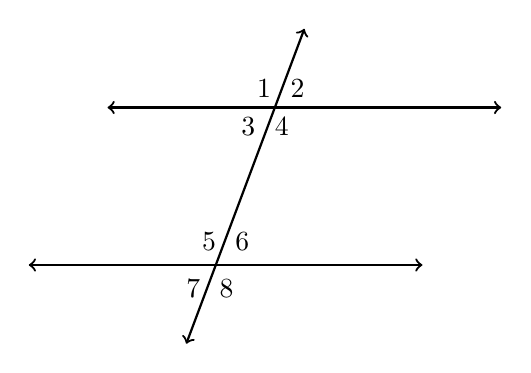
\begin{tikzpicture}[scale=1]
      \draw [<->, thick] (3,2)--(8,2);
      \draw [<->, thick] (2,0)--(7,0);
      \draw [<->, thick] (4,-1)--(5.5,3);
      \node at (4.5,0.3) [left]{$5$};
      \node at (4.5,0.3) [right]{$6$};
      \node at (4.3,-0.3) [left]{$7$};
      \node at (4.3,-0.3) [right]{$8$};
      \node at (5.2,2) [above left]{$1$};
      \node at (5.2,2) [above right]{$2$};
      \node at (5,2) [below left]{$3$};
      \node at (5,2) [below right]{$4$};
    \end{tikzpicture}
  \end{multicols}

\newpage
\item Given two parallel lines and a transversal, as shown. Write down each value, given that $m\angle 5 =  120^\circ$.
  \begin{multicols}{2}
    \begin{enumerate}[itemsep=0.5cm]
      \item $m\angle 3 = $
      \item $m\angle 2 = $
      \item $m\angle 4 = 2x$. Find $x$
    \end{enumerate}
      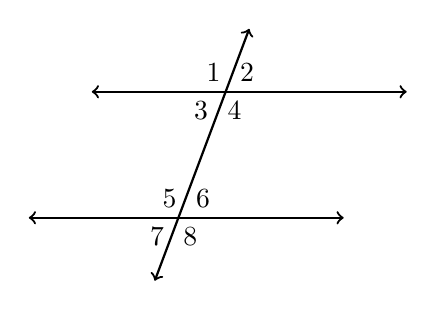
\begin{tikzpicture}[scale=0.8]
      \draw [<->, thick] (3,2)--(8,2);
      \draw [<->, thick] (2,0)--(7,0);
      \draw [<->, thick] (4,-1)--(5.5,3);
      \node at (4.5,0.3) [left]{$5$};
      \node at (4.5,0.3) [right]{$6$};
      \node at (4.3,-0.3) [left]{$7$};
      \node at (4.3,-0.3) [right]{$8$};
      \node at (5.2,2) [above left]{$1$};
      \node at (5.2,2) [above right]{$2$};
      \node at (5,2) [below left]{$3$};
      \node at (5,2) [below right]{$4$};
    \end{tikzpicture}
  \end{multicols}
  
\newpage
\item Given two parallel lines and a transversal, with alternate interior angles $m\angle 4 = 5x$ and $m\angle 5 = 2x + 40$. Write an equation, then solve for $x$.
\begin{flushright}
  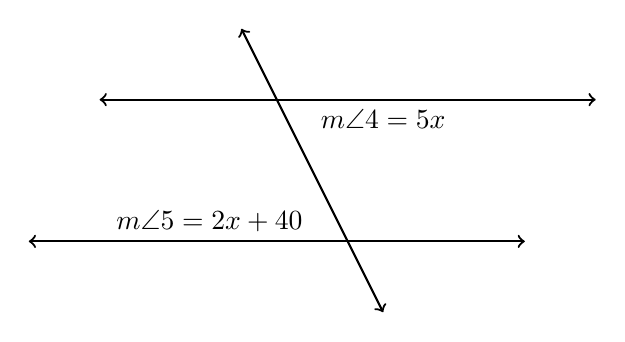
\begin{tikzpicture}[scale=0.9]
    \draw [<->, thick] (0,0)--(7,0);
    \draw [<->, thick] (1,2)--(8,2);
    \draw [<->, thick] (5,-1)--(3,3);
    %\draw [<->, thick] (11,-1)--(9,3);
    %\node at (4, 1.7){$1$};
    \node at (5, 2)[below]{$m\angle 4 = 5x$};
    \node at (4, 0)[above left]{$m\angle 5 = 2x + 40$};
    %\node at (10, 0.25){$3$};
  \end{tikzpicture}
  \end{flushright}

\newpage
\item Two parallel lines intersect a transversal, shown. Given the same-side interior angles  $m\angle 4 = 16x - 79$ and $m\angle 6 = 6x + 50$. Solve for $x$ then find the measure of $\angle 4$. 
  \begin{flushright}
    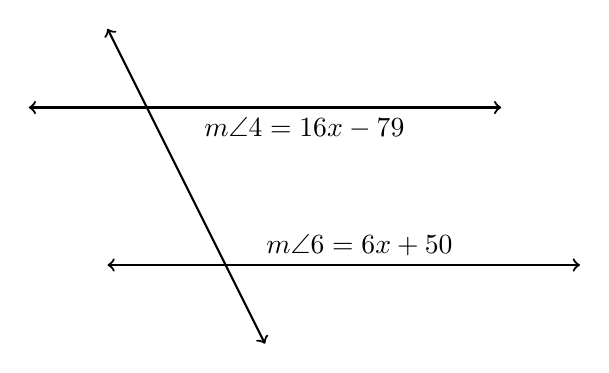
\begin{tikzpicture}[scale=1]
      \draw [<->, thick] (3,0)--(9,0);
      \draw [<->, thick] (2,2)--(8,2);
      \draw [<->, thick] (5,-1)--(3,3);
      %\draw [<->, thick] (11,-1)--(9,3);
      %\node at (4, 1.7){$1$};
      \node at (5.5, 2)[below]{$m\angle 4 = 16x - 79$};
      \node at (6.2, 0.25){$m\angle 6 = 6x + 50$};
      %\node at (10, 0.25){$3$};
    \end{tikzpicture}
    \end{flushright}

\newpage
\item Given parallel lines $\overleftrightarrow{AB} \parallel \overleftrightarrow{CF}$, $m\angle BAE=75^\circ$ and $m\angle DAE=55^\circ$. \\[0.5cm]
  Find $m\angle ADC = x$ and $m\angle AEF = y$.
  \begin{flushright}
  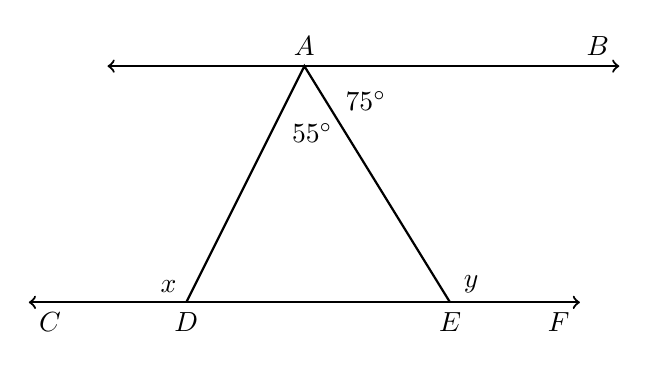
\begin{tikzpicture}[scale=1.]
    \draw [<->, thick] (0,3)--(6.5,3) node[above left]{$B$};
    \draw [<->, thick] (-1,0) node[below right]{$C$}--
      (5,0)--
      (6,0) node[below left]{$F$};
    \draw [-, thick] (1,0) node[below]{$D$}--
      (2.5,3) node[above]{$A$}--
      (4.35,0) node[below]{$E$};
    \node at (2.6,2.4)[below]{$55^\circ$};
    \node at (2.9,2.8)[below right]{$75^\circ$};
    \node at (1,0)[above left]{$x$};
    \node at (4.4,0)[above right]{$y$};
  \end{tikzpicture}
  \end{flushright}

    
\end{enumerate}
\end{document}